%%%%%%%%%%%%%%%%%%%%%%%%%%%%%%%%%%%%%%%%%%%%%%%%%%%%%%%%%%%
% EPFL report package, main thesis file
% Goal: provide formatting for theses and project reports
% Author: Mathias Payer <mathias.payer@epfl.ch>
%
% This work may be distributed and/or modified under the
% conditions of the LaTeX Project Public License, either version 1.3
% of this license or (at your option) any later version.
% The latest version of this license is in
%   http://www.latex-project.org/lppl.txt
%
%%%%%%%%%%%%%%%%%%%%%%%%%%%%%%%%%%%%%%%%%%%%%%%%%%%%%%%%%%%
\documentclass[a4paper,11pt,oneside]{report}
% Options: MScThesis, BScThesis, MScProject, BScProject
\usepackage[MScThesis,lablogo]{EPFLreport}
\usepackage{xspace}
\usepackage{listings}
% Enable all todo comments.
\usepackage[]{todonotes}
% Uncomment this to disable the comment blocks
% \usepackage[disable]{todonotes} 
% This is how we do comments for papers in the lab. This way you can see it 
% both in TeX and when you compile the PDF. Make sure they're all removed for 
% the final version by switching the lines above. I also don't mind if you 
% delete them once resolved because I can see them changed in git :)
\newcommand{\ant}[1]{\todo[inline,color=blue!40]{Antony: #1}}
\newcommand{\dam}[1]{\todo[inline,color=red!40]{Damian: #1}}
\newcommand{\lou}[1]{\todo[inline,color=green!40]{Louis: #1}}

\lstset{ 
  basicstyle=\footnotesize,
  frame=single,
  language=C++,
}

\title{Recovering type information from compiled binaries\\to aid in 
instrumentation}
\author{Louis Merlin}
\supervisor{Antony Vennard}
\adviser{Prof. Dr. sc. ETH Mathias Payer}
%\coadviser{Second Adviser}
\expert{Damian Pfammatter}

\newcommand{\sysname}{FooSystem\xspace}

\setlength{\parindent}{0cm}

\begin{document}
\maketitle
\makededication
\makeacks

\begin{abstract}
% The abstract serves as an executive summary of your project.
% Your abstract should cover at least the following topics, 1-2 sentences for
% each: what area you are in, the problem you focus on, why existing work is
% insufficient, what the high-level intuition of your work is, maybe a neat
% design or implementation decision, and key results of your evaluation.

The analysis of closed-source C++ programs is an arduous task.
C++ adds several powerful functionalities to the C language, which leads to
complex binaries.

Knowledge of class types and hierarchies can prove valuable during the reverse
engineering process.
Fortunately, some of that information can be recovered from stripped binaries
due to the way polymorphism is implemented in C++ compilers.

With \emph{dis-cover}, the tool we developed, we extract \emph{class
information} and the \emph{hierarchy tree} from a stripped C++ binary, and
write DWARF debug information and symbols for the later use of that knowledge
by any existing debugging tool.
Through this method, we aim to demonstrate an open and collaborative way of
writing static analysis tools.

By researching in detail the way C++ exceptions are implemented, we also
augment the capabilities of the \emph{RetroWrite} static rewriting tool to
support position-independent C++ binaries.
We also show how the class information extracted by dis-cover could be used to
improve the instrumentation done by RetroWrite.

By utilizing \emph{dis-cover}, we successfully extract useful information from
closed-source applications like Zoom.

We also detail the improvements now needed for \emph{RetroWrite} to support
rewriting closed-source stripped position-independent C++ binaries.

\end{abstract}

% \begin{frenchabstract}
% For a doctoral thesis, you have to provide a French translation of the
% English abstract. For other projects this is optional.
% \end{frenchabstract}

\maketoc

%%%%%%%%%%%%%%%%%%%%%%
\chapter{Introduction}
%%%%%%%%%%%%%%%%%%%%%%

% The introduction is a longer writeup that gently eases the reader into your
% thesis~\cite{dinesh20oakland}. Use the first paragraph to discuss the setting.
% In the second paragraph you can introduce the main challenge that you see.
% The third paragraph lists why related work is insufficient.
% The fourth and fifth paragraphs discuss your approach and why it is needed.
% The sixth paragraph will introduce your thesis statement. Think how you can
% distill the essence of your thesis into a single sentence.
% The seventh paragraph will highlight some of your results
% The eights paragraph discusses your core contribution.

% This section is usually 3-5 pages.

Work on C++ began in 1979, as a "C with classes"~\cite{cwithclasses}.
Since then, the language has grown in popularity, and even surpassed C 
itself~\cite{stackoverflowpopularity}.
Examples of well-known C++ projects include modern browsers like 
Chrome~\cite{chrome} and Firefox~\cite{firefox}, the Qt Framework~\cite{qt}, or 
the Zoom~\cite{zoom} conferencing software.
Nevertheless, most reverse-engineering efforts have been focused towards C
binaries, because analysis methods found this way are simpler and will often
work on C++ binaries too.

This has meant reverse engineering tools like Ghidra~\cite{ghidra}, IDA 
Pro~\cite{ida}, radare2~\cite{radare} or Binary Ninja~\cite{binja} have
treated non-C binaries as second-class citizen.
These tools will often show C++ specific features as passing comments, failing 
to show the real implications of a try/catch block or a polymorphic class.
The complexity of C++ has also lead binary rewriters like
RetroWrite~\cite{dinesh20oakland} to focus on C binaries only, leaving a whole
ecosystem of binaries unstudied.

The blame can mostly be put on the complexity of C++ when compared to C.
Whereas C translates quite naturally to assembly, abstractions specific to C++ 
require more work and complexity to be translated to assembly.
This also leads to important information being lost from C++ source code to 
binary, but also certain information remaining, like run-time type information.

In this thesis we would like to present the 
\emph{dis-cover}~\cite{discovergithub} static analysis tool.
This tool extracts class hierarchy information from a C++ binary, and
re-injects it into the binary as debug information using the DWARF format.
This enables other debugging tools to see and display this information.

This class hierarchy information is included in the binary for functionality
reasons, and is even kept after basic stripping of the program.
Several large closed-source projects, like the Zoom conferencing software,
have several thousands of classes linked to each other in complex class
hierarchy trees.
Having that information easily accessible would help reverse engineering
efforts.

The recent RetroWrite~\cite{dinesh20oakland} project by the HexHive lab is a 
static rewriting tool for unstripped x86\_64 position-independent binaries.
It enables the instrumentation of projects when we do not have access to the 
source code.
Instrumentation is the process of adding instructions to a binary, to add
additional security checks for example.
The target can be a legacy project, a closed-source product or even malware.
In this thesis we will also detail our improvements to RetroWrite to support
unstripped position-independent \emph{C++} binaries, and the possibilities
opened by this feature for future researchers.

%%%%%%%%%%%%%%%%%%%%
\chapter{Background}
%%%%%%%%%%%%%%%%%%%%

% The background section introduces the necessary background to understand your
% work. This is not necessarily related work but technologies and dependencies
% that must be resolved to understand your design and implementation.

% This section is usually 3-5 pages.


\section{Executable and Linkable Format (ELF)}

The common standard \emph{Executable and Linkable Format} (ELF) format is 
mostly used as executable files, object code and shared libraries.
It is the current standard format for executable files on UNIX
systems~\cite{elfstandard}.

An ELF file contains a program header table, which describes memory segments 
(e.g. "this is read-only data", "this is executable instructions").
It also usually contains a section header table, describing sections (their 
name, size, offset and some flags).
Memory segments contain information that is used at runtime, while sections
contain relocation and linking information.

The rest of an ELF file is taken up by different sections.
Famous sections include
\texttt{.text} (where the instructions are),
\texttt{.data} (where you will see global tables and other variables),
\texttt{.rodata} (you will find strings in here)
and \texttt{.eh\_frame} (where exception unwinding information is stored for 
C++ binaries).


\section{Position-Independent Code (PIC) and Executable (PIE)}
\label{picpie}

Position-independence for code is a property that guarantees that code will 
execute correctly no matter the base address of the body of code.
This is made possible by computing \emph{relative positions} instead of
using base addresses, as well as a feature called \emph{relocations}.

PIC is most often found for shared libraries, so that they can be loaded and
shared by any number of processes without breaking offsets, or even thinking
about them.
PIE binaries are seen as more secure because they allow for easy inserting of 
security measures like address space layout 
randomization~\cite{aslr}.
We will talk more about PIE in \autoref{retrowritesection}.


\section{C++ features}

\subsection{Polymorphism}
\label{polymorphism}

The C++ programming language implements polymorphism.
This feature enables complex code logic that can comply with external business 
logic.
Here we will introduce the example that will follow us throughout this thesis :
in \autoref{classes} we define two abstract base classes \emph{Animal} and 
\emph{Feline},
and the two classes \emph{Cat} (that inherits from Animal and Feline) and 
\emph{Dog} (that inherits from Animal).
In a large code base, with multiple teams of programmers working on different 
features,
an Animal could be passed around without caring about whether it was a Cat, a 
Dog or any other species.
This Animal is sure to overwrite the \emph{speak} method and have whatever 
other properties and methods Animal has defined.
This logic is verified by the compiler.

\begin{figure}
\begin{lstlisting}
#include <iostream>
#include <string.h>

using namespace std;


class Animal {
public:
  virtual void speak() {}
};

class Feline {
public:
  virtual void retract_claws() {}
};

class Cat : public Animal, public Feline {
public:
  virtual void speak() { cout << "Purr" << endl; }
};

class Dog : public Animal {
public:
  virtual void speak() { cout << "Woof" << endl; }
};


int main (int argc, char *argv[]) {
  Animal *my_animal = nullptr;

  if (argc == 2) {

    // We can instantiate an instance of a subclass into a pointer of type
    // Animal*.
    if (strcmp("cat", argv[1]) == 0) {
      my_animal = new Cat();
    } else if (strcmp("dog", argv[1]) == 0) {
      my_animal = new Dog();
    } else {
      return 1;
    }

    my_animal->speak();

    // We can dynamic_cast an Animal* into a Feline*, even though one does not
    // inherit from the other (but Cat inherits from both).
    Feline *my_feline = dynamic_cast<Feline*>(my_animal);
    if (my_feline) {
      my_feline->retract_claws();
      cout << "This feline could retract its claws" << endl;
    }
  }

  return 0;
}
\end{lstlisting}
\caption{Polymorphic classes in C++}
\label{classes}

\end{figure}

This polymorphism feature also enables re-use of functionality by inheriting 
parent classes.
If you want to implement a Lemur and your Animal class already has an 
implementation of the eat method,
you don't need a lemur-specific implementation if appropriate. 

Polymorphic classes are defined by having at least one virtual method, which is 
inheritable and overridable.
With this polymorphism comes type conversion, of which there are two kinds.
The first, \emph{static\_cast}~\cite{staticcast}, will check that the
conversion is upcasting at compile time,
but does not do any runtime checks to verify the validity of the conversion.
An example of upcasting is converting a pointer of a \emph{Cat} to a pointer
of an \emph{Animal}.
The fact that a class is polymorphic will have no impact on this type of 
casting.
The second is the more interesting one for us. It is the 
\emph{dynamic\_cast}~\cite{dynamiccast} expression.
Dynamic casting is a safe kind of type conversion that can handle downcasting 
and sidecasting.
An example of downcasting is converting a pointer of an \emph{Animal} to a
pointer of a \emph{Cat}. This is not guaranteed to work.
An example of sidecasting is converting a pointer of an \emph{Animal} to a
pointer of a \emph{Feline}. This is also not guaranteed to work (if the
Animal pointer was that of a Dog for example).
In order to achieve a dynamic cast, the system must have some kind of
information about the object's data type at runtime.

This is where \emph{Run-Time Type Information} (RTTI) comes into the picture.
The system will use this RTTI to infer type inheritance for dynamic casting.
We will now go into implementation details of RTTIs and \emph{virtual tables}
(vtables), which point to them.

To make vtables and RTTIs appear in your C++ binary, you will need to define
classes that inherit from each other, as well as at least one virtual method
in one of these classes.
\autoref{classes} shows an example of such classes.
You will also need to instantiate these classes, and have some logic to make
the class logic runtime dependent. 
This is extremely common in practice, as it is the core motivation for
polymorphism in the first place.
For an example, see the conditional creation of the my\_animal variable, as
well as dynamic cast between Animal and Feline we defined in \autoref{classes}.
If you do not do one of these things, the class logic is likely to be abstracted
away by the compiler for optimization reasons.

\begin{figure}

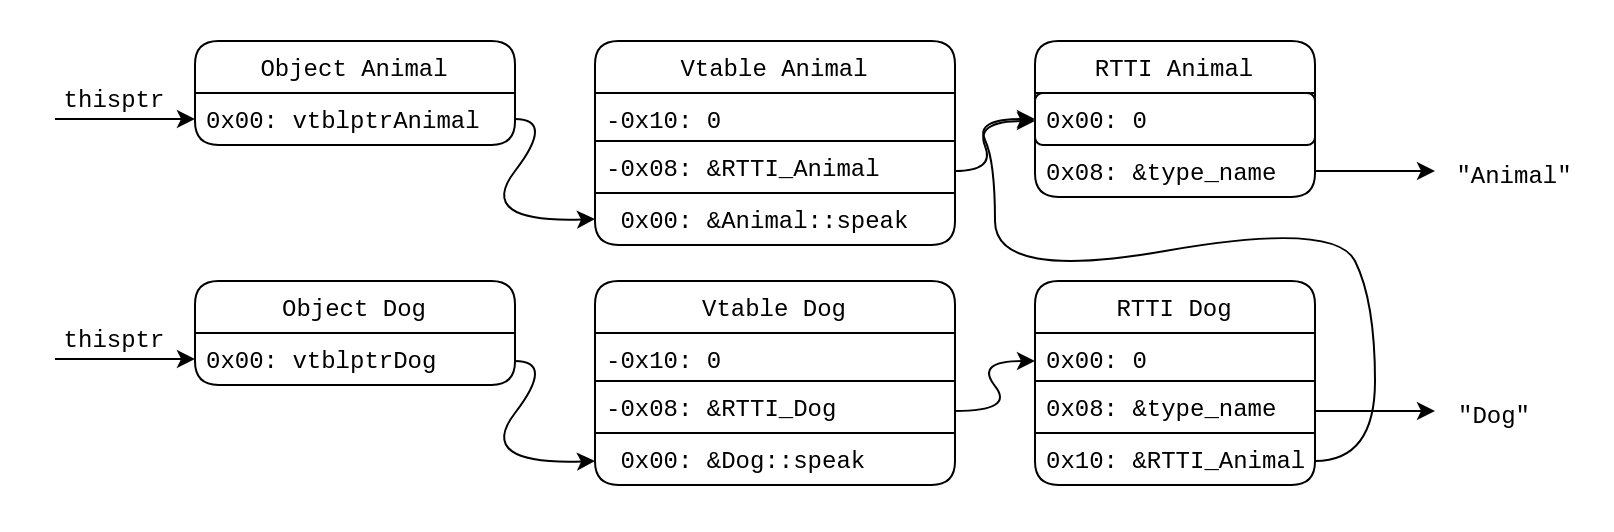
\includegraphics[width=16cm]{RTTI_graph.png}
\caption{Overview of an example of vtables and RTTI in memory}
\label{rttigraph}

\end{figure}

The structure of vtables and RTTIs is detailed in \autoref{rttigraph}.
All of this is defined in the Itanium C++ ABI~\cite{cppabi}.
An instance of a virtual class Animal will contain the \emph{vtblptrAnimal}, 
a pointer to the \emph{virtual table} (vtable) for the Animal class.
This vtable will be shared by all instances of this class (even by instances
of a class that inherits from Animal), and will contain pointers to the virtual
methods of the class.
The first value preceding the vtable is a pointer to the RTTI of the class. A
program finds out the class inheritance of a class instance at runtime by
following this pointer.

The RTTI itself is composed of a pointer to a vtable for the typeinfo class
(defined by the compiler) as well as a pointer to the type name (this type 
name is not removed by simple stripping of the binary, like with 
\emph{objdcopy --strip-all}).
This name is mangled using C++ mangling, and can trivially be demangled.
Here are some examples of C++ name mangling :
\emph{\_ZTI6Feline} demangles to \emph{typeinfo for Feline};
\emph{\_ZTV6Feline} demangles to \emph{vtable for Feline}.
Mangling is especially useful when defining several methods in the same scope 
with different arguments (this is called overloading), in order to
differentiate the different methods.
Mangling is also useful because of special characters in class names, like the
\emph{::} characters who separate namespaces.
The next values of the RTTI are pointers to the RTTIs of the parent classes.
These are used at runtime to check the relationship between classes.
See \autoref{rttigraph} for an example, with the Dog RTTI containing a pointer 
to the Animal RTTI.

\subsection{Exceptions}
\label{exceptions}

Exceptions are one of the defining features that make C++ stand out from C.
In contrast to C errors, which terminate the whole program, C++ exceptions
can be caught and handled.

In order for the program to continue execution after an exception is caught,
binaries need some way of safely doing \emph{stack unwinding}.
This means that the systems needs to restore the stack variables to the state
they were before entering the try block.

The information on how to safely unwind the stack is stored in the
\texttt{.eh\_frame} section. It is encoded in a format similar to DWARF data
(see \autoref{dwarf}).

The system also needs to safely release memory that is outside of the scope
reached after an exception is caught.
See \autoref{unwinding} for an example of code that will only guarantee safety
if there is this mechanism in place.

\begin{figure}
\begin{lstlisting}
#include <iostream>

using namespace std;


void this_method_might_throw(int x) {
  // This buffer is instantiated.
  char* this_object_could_leak = new char[1024];

  // If the throw is called, the buffer will stay instantiated if there is
  // no stack unwinding.
  if (x) throw runtime_error(":explosion:");

  // If the throw is not called, we free the buffer ourselves.
  delete [] this_object_could_leak;
}

int main() {
  try {
    this_method_might_throw(10);
  } catch (const exception& e) {
    return 1;
  }
  // Thanks to stack unwinding, we can be sure that the buffer from
  // this_method_might_throw was freed and will not leak.
  return 0;
}
\end{lstlisting}
\caption{Example of C++ exception throwing and catching to illustrate stack 
unwinding}
\label{unwinding}

\end{figure}

\begin{figure}
\begin{lstlisting}
	.section	.gcc_except_table,"a",@progbits
	.p2align	2
GCC_except_table2:

.Lexception1:
	.byte	255                     # @LPStart Encoding = omit
	.byte	3                       # @TType Encoding = udata4
	.uleb128 .Lttbase0-.Lttbaseref0

.Lttbaseref0:
	.byte	1                       # Call site Encoding = uleb128
	.uleb128 .Lcst_end1-.Lcst_begin1

.Lcst_begin1:
	.uleb128 .Ltmp3-.Lfunc_begin1   # >> Call Site 1 <<
	.uleb128 .Ltmp4-.Ltmp3          #   Call between "try" and "catch"
	.uleb128 .Ltmp5-.Lfunc_begin1   #     jumps to .Ltmp5 (cleanup function)
	.byte	1                       #   On action: 1

	.uleb128 .Ltmp4-.Lfunc_begin1   # >> Call Site 2 <<
	.uleb128 .Lfunc_end2-.Ltmp4     #   Call after "catch"
	.byte	0                       #     has no landing pad (do nothing)
	.byte	0                       #   On action: cleanup

.Lcst_end1:
	.byte	1                       # >> Action Record 1 <<
                                        #   Catch TypeInfo 1
	.byte	0                       #   No further actions
	.p2align	2
                                        # >> Catch TypeInfos <<
	.long	_ZTISt9exception        # TypeInfo 1 (what we are catching)
\end{lstlisting}
\caption{Assembly representation of an except\_table for a simple program}
\label{excepttable}
\end{figure}

This memory safety logic is defined in a table called the \emph{Language
Specific Data Area}, in a section of the binary called the
\texttt{.gcc\_except\_table}~\cite{airsexcepttable}.
In theory this section should be language specific, but in practice the
implementation is the same for every language when using the \emph{GNU
Compiler Collection}~\cite{gcc} (GCC), that supports languages like
Objective-C, Fortran or Go, and when using \emph{LLVM}~\cite{llvm}, that
supports most well-known compiled languages.

In figure \autoref{excepttable} you can see a \texttt{.gcc\_except\_table} that 
was generated from the code in \autoref{unwinding}. We will now go through line
by line to explain the inner workings of this table.
This will help us explain why they are so important, and later why we had to
rewrite them (see \autoref{retrowritedesign})

The first three lines define that "this is an except table starting".

The following seven lines define the parameters of this except table.
These are, for example, the encoding of the values present in the table (the
\texttt{.byte 3} and \texttt{.byte 1} lines), or the length of the table (the
\texttt{.uleb128 .Lcst\_end1-.Lcst\_begin1} line).

Next, we have the beginning of the call site table at \texttt{Lcst\_begin1}.
The first call site defines that if an exception is thrown while executing
instructions between the "try" and "catch blocks (here defined as the
\texttt{Ltmp3} and \texttt{Ltmp4} labels), then you see if it matches
\emph{action 1} before jumping to the landing pad (here \texttt{Ltmp5}).

The actions are defined under the call site table, in the action table. You
can see them defined at the \texttt{Lcst\_end1} label.
The first action is defined as "catch TypeInfo 1". The TypeInfos are defined
bellow the actions, as a list of pointers to the different exceptions we might
be catching. Here, typeinfo 1 is a simple "exception", which matches with our
C++ code.

Coming back to the first call site : the landing pad of this call site is, in
this case, a pointer to code that will free and clean up the buffers and
variables that might have been instantiated.

Quite interestingly, the "TypeInfo" types are checked against the
\emph{Run-Time Type Information} (RTTI) we talked about in the previous
subsection.
We will have more to say about RTTIs in the following chapters.

\subsection{Global constructors and frame dummy}
\label{framedummy}

During the execution of an ELF file, some methods will be run before the main
program starts. Pointers to these methods are stored in the
\texttt{init\_array}.
A simple C++ binary that uses exceptions will have an initialization array
containing a pointer to the \texttt{frame\_dummy}. This method is in charge of
setting up the stack frames to unwind the frame during exception handling
later on.
In the initialization array, you will also find pointers to a global
constructor for every compilation unit (usually, a compilation unit is a C++
source file).


\section{DWARF debugging standard}
\label{dwarf}

\emph{DWARF} is the debugging standard used widely in conjunction with 
executable ELF files.
It is often included in these ELF files in the \texttt{.debug\_info} section 
(and other related sections).
This debug information is made up of Debugging Information Entries 
(\emph{DIEs}).
These entries can contain information about variable names, method definitions, 
the compilation process, or more importantly for us, class names and class 
inheritance. You can also map source code to binary code.
All of this information is usually used in debuggers.

The \texttt{.eh\_frame} section mentioned in \autoref{exceptions} is also used
by debuggers to unwind the stack for debugging purposes.
It gives information to identify where to catch exceptions, as well as what
destructors to call while unwinding the stack.

DWARF data takes the form of a tree of values.
The root of the tree is called the \emph{Compile Unit} (CU).
It contains information about the source code file, the programming language
used as well as the compiler.


\section{RetroWrite} \label{retrowritesection}

The \emph{RetroWrite}\cite{dinesh20oakland} project is a project from the
HexHive lab that aims to statically rewrite binaries and instrument them, to
improve fuzzing capabilities, or retrofit security measures.
Static binary rewriting is the process of taking a binary file, and modifying
it such that there is a patch applied to it but the other functionalities
remain the same.

RetroWrite's core idea is to symbolize all of the addresses in the machine
code. This means transforming an address offset (+8) into a symbol
(.LD1234) and adding the appropriate label at that location.
These labels will be used by the assembler to compute the addresses of
functions and data offsets for example.
This way, we can add any instruction after and before existing instructions
without breaking relative offsets.

RetroWrite only works on \emph{x86\_64} unstripped position-independent
executables (see \autoref{picpie}), compiled from C.
This enables the RetroWrite to stay heuristics-free (meaning that it is
designed to work for every example without exceptions).

If you try to rewrite a binary that is stripped, the code blocks that
correspond to functions will not be identified as such.
RetroWrite currently needs to know the function boundaries to rewrite a binary.
Identifying the function boundaries would require heuristics.

If you try to rewrite a binary that is not position-independent, the
positions (pointers) in your binary are indistinguishable from data, and it
becomes an unsolvable problem to differentiate between data and a pointer,
which is why you would also need heuristics in that scenario.


%%%%%%%%%%%%%%%%
\chapter{Design}
%%%%%%%%%%%%%%%%

% Introduce and discuss the design decisions that you made during this project.
% Highlight why individual decisions are important and/or necessary. Discuss
% how the design fits together.

% This section is usually 5-10 pages.


\section{dis-cover}

The primary goal of this project was to extract some debug information from a
stripped C++ binary, make it available through DWARF in order to use that
information in other projects, as a proof of concept.
The hope is that this process will be re-used in other projects in the future.
For this project, we decided to focus on recovering class information from
\emph{Run-Time Type Information} (RTTI, see \autoref{polymorphism}).

% Design => Decisions
% We decided not to reproduce Marx's work
% First attempt : recover classes from RTTI
% Future work : could take approaches like Marx and re-feed it like us
Class recovery from compiled C++ binaries has been tried multiple ways before:
there are plugins for popular debugging tools, like 
ida\_gcc\_rtti~\cite{idagccrtti} for IDA Pro (which requires a license),
or Ghidra-Cpp-Class-Analyzer~\cite{ghidracppclassanalyzer} for Ghidra
(but this information is only usable inside of the Ghidra debugger);
there are academic projects such as MARX~\cite{marx} that rely on heuristics 
around vtables to find classes and inheritance information.
The MARX project can recover classes when no RTTI is present (in the Chrome 
project for example, where the \emph{-fno-rrti} compilation flag is used),
with around 90\% accuracy.

\subsection{Finding Run-Time Type Information}

As we mentioned in the Background chapter, the RTTIs are available for a
class hierarchy tree when there is at least one virtual method implemented
by one of the classes.
We decided to test if RTTIs occurred often in the wild : we proceed to download 
every Debian package that listed C++ as a dependency (get the list with 
\emph{apt-cache rdepends libgcc1} on a Debian machine).
Out of around 80'000 packages, 5827 of them list C++ as a dependency.
Out of those, we extracted classes from 3194 (54\%).
This does not mean that the other 46\% of packages do not use classes,
because in many cases these classes are optimized away by the compiler
(in the more straightforward cases).
We will share more details about this experiment in \autoref{debiansection}.

When looking at a binary's vtables and RTTIs, we only need to look for a
specific subset of them : the primary base virtual tables and their RTTIs.
There is one for each class defined in the binary. Secondary virtual
tables occur when there is multiple inheritance and complex method overwrites.
They define only a subset of a class' methods, and may not contain RTTIs.
We can differentiate the two kinds of virtual tables by the presence of an
offset at the beginning of the vtable : a primary base virtual table will have
a value of $0$ as an offset, whereas a secondary virtual table will have an
offset to the primary base virtual table. See
\autoref{multipleinheritancegraph} for a visual example of RTTIs and vtables
in a multiple inheritance scenario.

\begin{figure}

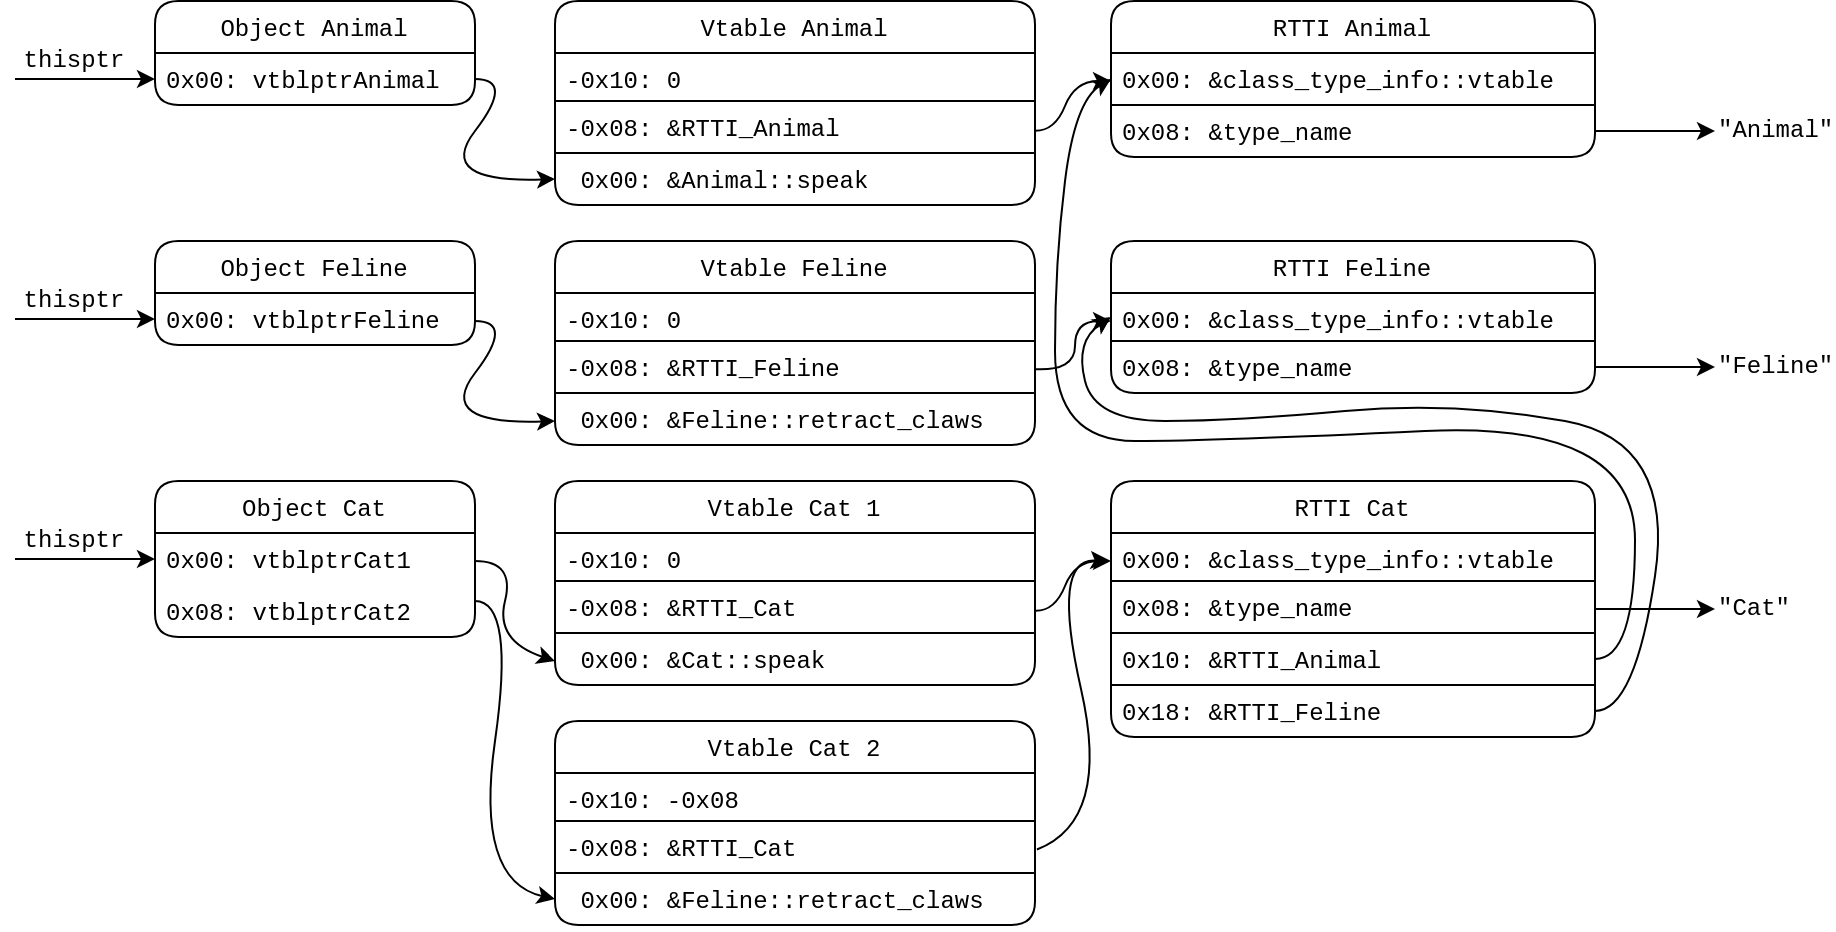
\includegraphics[width=16cm]{Feline.png}
\caption{Overview of an example of vtables and RTTI in memory with multiple 
inheritance}
\label{multipleinheritancegraph}

\end{figure}

\subsection{DWARF}
\label{dwarfdesign}

Once we have extracted class information from RTTI, next comes the question :
what should we do with all of this class information ? What would be the most
useful format to output the data in ?
This is where DWARF~\cite{dwarf} comes in the picture. DWARF is the debugging 
standard for UNIX programs.
It is mostly used by developers trying to understand where their implementation 
fails,
and by reverse engineers to get a better understanding of how a program was 
conceived (although DWARF information is usually stripped from proprietary 
software).
This kind of debug data is mostly found in compiled binaries, written in C,
C++ or Rust for example. 
By having DWARF data as an output, the information would become readable by 
most modern reversing tools.

There is a current push for DWARF to become the lingua franca for reverse 
engineering tools, lead by researchers like Dr. Sergey Bratus~\cite{bratus} 
from DARPA.
He has published a paper in 2011 where he exploits certain features of DWARF to
control program execution : Exploiting the hard-working
DWARF~\cite{hardworkingdwarf}.
In it, they prove that the DWARF information used during exception handling
is Turing-complete and can be used to embed exploits in executables.

DWARF data is structured as a tree of \emph{Debug Information Entries} 
(DIEs). These entries contain a \emph{tag} and a list of
\emph{attributes}.
These entries can describe how the original code is written, as well as
information about classes, variables, types, and other structures in the
binary. \autoref{dwarfdies} shows an example of such entries, describing
pointers and methods in a simple program. Lines beginning with \emph{DW\_TAG}
describe the type of the debug information entry, and the following lines
beginning with \emph{DW\_AT} describe the attributes of this entry.

\begin{figure}
\begin{lstlisting}
< 1><0x00001d94>    DW_TAG_class_type
                      DW_AT_containing_type       <0x00001d94>
                      DW_AT_calling_convention    DW_CC_pass_by_reference
                      DW_AT_name                  Animal
                      DW_AT_byte_size             0x00000008
                      DW_AT_decl_file             0x00000022 /tmp/animals.cpp
                      DW_AT_decl_line             0x00000006
< 2><0x00001da1>      DW_TAG_member
                        DW_AT_name                  _vptr$Animal
                        DW_AT_type                  <0x00001dd2>
                        DW_AT_data_member_location  0
                        DW_AT_artificial            yes(1)
< 2><0x00001dab>      DW_TAG_subprogram
                        DW_AT_linkage_name          _ZN6Animal5speakEv
                        DW_AT_name                  speak
                        DW_AT_decl_file             0x00000022 /tmp/animals.cpp
                        DW_AT_decl_line             0x00000008
                        DW_AT_virtuality            DW_VIRTUALITY_virtual
                        DW_AT_declaration           yes(1)
                        DW_AT_external              yes(1)
                        DW_AT_accessibility         DW_ACCESS_public
                        DW_AT_containing_type       <0x00001d94>
\end{lstlisting}
\caption{Extract of a dwarfdump output showing pointers and methods}
\label{dwarfdies}
\end{figure}

The DWARF format also uses abbreviations to compress the debug information.
Instead of re-describing a DIE every time, their structure is defined in an
abbreviation table (stored in the \emph{debug\_abbrev} section of the ELF
file).
Each DIE will have an index in that table, which describes its tag and list
if attributes names and types. The rest of the DIE is the list of its
attributes, in the order they were defined in the abbreviation.

In this project, we use very minimalist DIE abbreviations, containing only
what we could infer from the analysis.

With dis-cover, we inject information in the debug and symbol sections of the
binary, creating a new ELF file with all of this useful info included.
We will go more into the implementation details in 
\autoref{wrappingimplementation}.

\subsection{Exceptions}

Exceptions are often implemented as classes, and dis-cover will naturally 
recover information about programmer-defined exceptions.
Future extensions of this work might consider recovering more information about 
exceptions.

We had to study and work with exceptions and exception handling frames for 
the augmentation of RetroWrite with C++ capabilities
(see \autoref{retrowriteimplementation}, \autoref{retrowritedesign} and
\autoref{exceptions} for more details).


\section{RetroWrite}
\label{retrowritedesign}

Today, RetroWrite supports the reversing of \emph{x86\_64}
position-independent binaries.
There was also work to augment RetroWrite to support kernel 
code~\cite{rwkernel} and \emph{arm\_64}~\cite{rwarm}.
We aimed to add C++ capabilities for \emph{x86\_64} binaries only, as it is
the most widely used platform (though the same logic will most probably apply
with a little tweaking to \emph{arm\_64} and other architectures).

The first bug we encountered while trying to use RetroWrite on C++ binaries
was due to the fact that the \emph{initialization array} (see
\autoref{framedummy}) contained a pointer to the \emph{frame dummy} and this
was not handled well during RetroWrite's symbolization process.
By adding special treatment for that scenario, we resolved this failure (see
more details in \autoref{fixinginitarray}).

Once that was fixed, we saw that using RetroWrite on binaries that had C++
exception handling would cause crashes in the new binary, caused by the fact
that the exceptions thrown were never caught.
Exception behavior is described in the \emph{Language Specific Data Area}
(LSDA), which is found in the \texttt{.gcc\_except\_table} section of the ELF
file.
This LSDA describes, row by row, actions to take for specific instruction in
the code we are hitting while dealing with a thrown exception. These actions
could be : destructing an out-of-scope variable, or examining a catch clause
to see if they should catch the current exception. See \autoref{exceptions}
for an example of this process.

We had to rewrite the LSDA in our new assembly representation, with the
appropriate labels and values, in order to make the exceptions work as they
should (see how we achieved that in \autoref{creatinglsda})

Once this was done, we were able to rewrite basic C++ binaries that used
exceptions.
% TODO modify this if it changes
Bigger projects still caused some issues, that will be addressed
before the code becomes public.


\section{Design for future integrations}

As described in \autoref{dwarfdesign}, we use the DWARF format as an output
for the extracted information. This makes the knowledge easily reusable in
other reverse engineering projects.

For example, dis-cover output could be used in RetroWrite in order to add
instrumentation around \emph{Object Type Integrity}, as defined in the CFIXX
paper~\cite{cfixx}, or reinforcing type checks as defined in the HexType
paper~\cite{hextype} to avoid type confusion errors and vulnerabilities.
See more details about these projects in \autoref{cfixx} and
\autoref{hextype}.

We also designed dis-cover in a heuristics-free way, which fits perfectly with
RetroWrite's current goal to avoid heuristics.

This heuristics-free design should not be an end goal though.
If later additions to RetroWrite were to improve its capabilities with
heuristics like those defined in the MARX paper for example (see
\autoref{relatedworksmarx}), it would only make the tool stronger and more
reliable.
The fact that we used the DWARF format as an output is what we consider the
most interesting part of the dis-cover tool.


%%%%%%%%%%%%%%%%%%%%%%%%
\chapter{Implementation}
%%%%%%%%%%%%%%%%%%%%%%%%

% The implementation covers some of the implementation details of your project.
% This is not intended to be a low level description of every line of code that
% you wrote but covers the implementation aspects of the projects.

% This section is usually 3-5 pages.

We decided to write a python module for this project, as the python ecosystem 
has great reverse engineering packages, and for easy integration in RetroWrite, 
which is also written in python.


\section{Finding RTTIs}

The first thing dis-cover does is find ELF sections where the vtables and RTTIs 
could be hiding.
This is usually \texttt{.rodata} (read-only data) and \texttt{.data.rel.ro}, 
but could sometimes also be related sections like \texttt{.data.rel.ro.local}, 
or \texttt{.rdata}.
As per the Itanium C++ ABI, the base vtable of a class will contain an 
"offset-to-top" at offset \emph{-0x10}, which will be 0 in the primary base 
virtual table's case, followed by a pointer to an RTTI at offset
\emph{-0x08}.
We simply have to pattern-match for zeroes directly followed by a pointer to 
another part of the read-only data sections, and we have a potential RTTI 
pointer. See \autoref{hexdump} for a hexdump of vtables and RTTIs in an ELF
file.

\lou{TODO label things as keys etc}

\begin{figure}

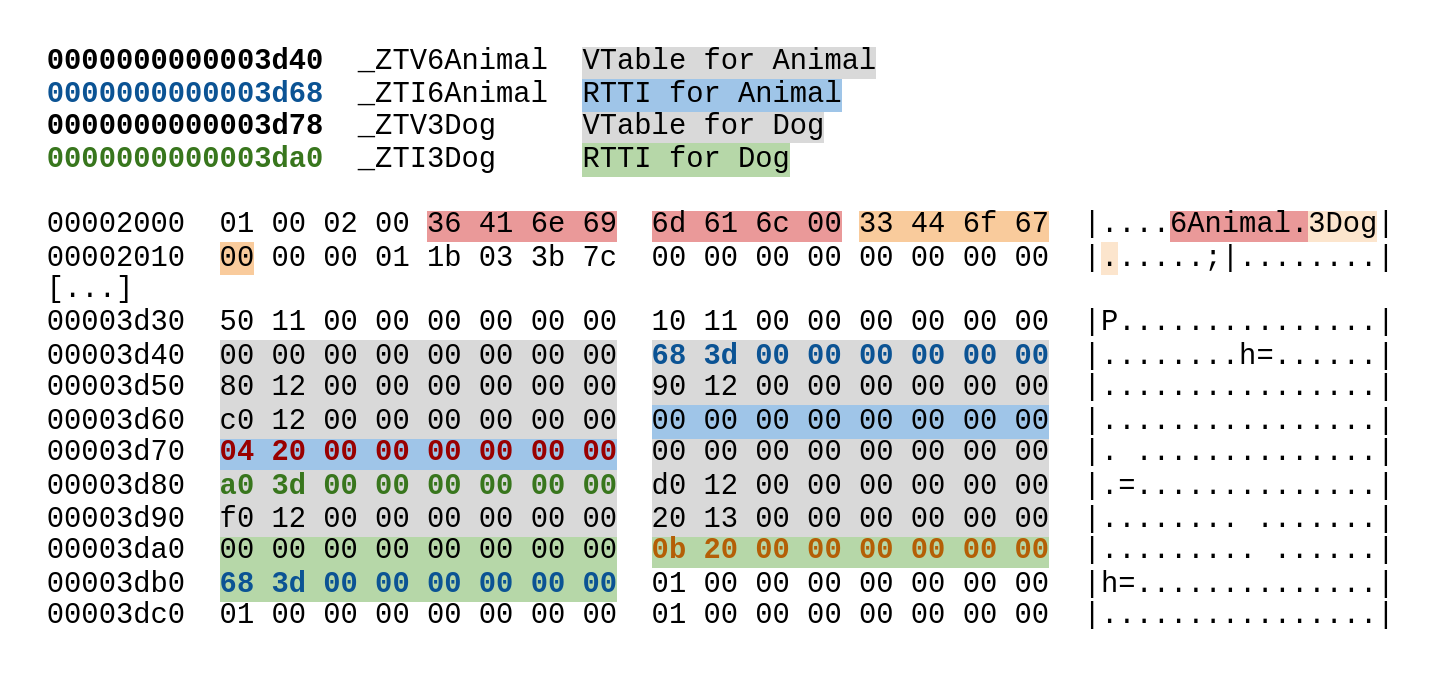
\includegraphics[width=16cm]{hexdump.png}
\caption{Hexdump of the location of vtables and RTTIs in an ELF file}
\label{hexdump}

\end{figure}

Next, we analyze the data at the pointer's value.
We check that we have not already extracted a class at that address, and if
not, we assert the following address is a pointer to a string located in a
read-only data section.
If it is, we can extract that string, demangle it, and we have a class name,
a virtual table address and an RTTI address that we have extracted.
The next values in the RTTI are pointers to the RTTIs the class inherits from.
We can go through them and parse them if we have not already, to add this 
inheritance information to the extracted class.

This algorithm is $O(n)$, as adding a class only adds one more value to parse.


\section{Creating DWARF data}
\label{dwarfimplementation}

Next, we want to add that information to the debug sections of a new ELF file.

In order to write DWARF data, the first step is defining the types we will be 
using, and their fields.
This is done by writing bytes in the \texttt{.debug\_abbrev} section.
For example, we create an abbrev of type \emph{class\_type}, which has a 
\emph{name}, and can have sub-field (children).
Then, we create the abbrev of type \emph{inheritance}, which has a 
\emph{type} (a reference to the parent type).

We can then populate the \texttt{.debug\_info} with classes and their 
inheritance data.
DWARF data takes the form of a tree of values. We have to create a 
\emph{compile\_unit} value at the root, and then the branches will be 
\emph{class\_type}s.
These \emph{class\_type}s will themselves have as children 
\emph{inheritance} values if the class inherits from another class.
\autoref{dwarfdump} shows a very simple example of this, with two class types 
and one inheriting from the other.

\begin{figure}
\begin{lstlisting}
< 1><0x0000001a>    DW_TAG_class_type
                      DW_AT_containing_type       <0x0000001a>
                      DW_AT_calling_convention    DW_CC_pass_by_reference
                      DW_AT_name                  Animal
                      DW_AT_byte_size             0x00000008
< 1><0x00000026>    DW_TAG_class_type
                      DW_AT_containing_type       <0x00000026>
                      DW_AT_calling_convention    DW_CC_pass_by_reference
                      DW_AT_name                  Dog
                      DW_AT_byte_size             0x00000008
< 2><0x00000031>      DW_TAG_inheritance
                        DW_AT_type                  <0x0000001a>
\end{lstlisting}
\caption{Extract of a dwarfdump output showing simple inheritance}
\label{dwarfdump}
\end{figure}

The strings themselves are stored in another section, \texttt{.debug\_str}, and 
are referred to with their offset in that section.


\section{Creating symbols}

Symbols are mainly used for shared object loading. To use the \emph{printf}
method from \emph{stdio.h} for example, the binary must be aware of a
method named \emph{printf}. The same is true for
\emph{system\_clock} in C++ for example.
Symbols are also used to have access to variable names, class names, function
names or any other kind of text information when debugging a binary.
In dis-cover, we want to create two symbols for every class we have found
during the analysis : one pointing to the vtable and one pointing to the RTTI,
and labeling them as such.

In order to create new symbol sections, we take the symbol table from the 
original binary (if there was one) and append the aforementioned symbols.

The two symbol sections are \texttt{.symtab}, which contains the information 
(offset, size, type, ...) for each symbol, and \texttt{.strtab}, which contains 
the strings related to these symbols.


\section{Wrapping things together}
\label{wrappingimplementation}

Once we have the three debug sections ready
(\texttt{.debug\_abbrev} with the debug types, \texttt{.debug\_info} with the 
debug information, and \emph{debug\_str} with the strings)
as well as the two symbol sections, we want to make them available to the user.
They contain all of the information we extracted from the binary.

We now have to go through a few hoops to make the debug and symbol information
available in one binary because these sections do not come alone : they have to
be accompanied by machine code and data.
We did not want to recreate a whole compiler to assemble all of this data.
Luckily, the \emph{eu-unstrip} tool was created as an utility application
to "combine stripped files with separate symbols and debug information".
\autoref{recovergraph} shows a diagram of the process we will explain in this
section.

\begin{figure}

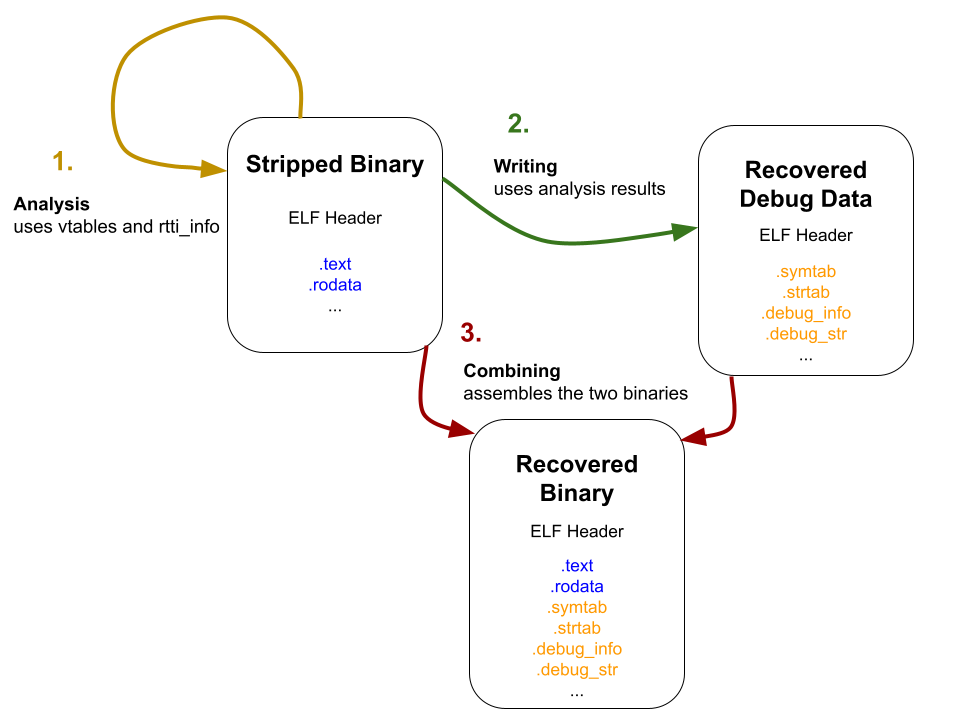
\includegraphics[width=16cm]{recover.png}
\caption{Combining the ELF files}
\label{recovergraph}

\end{figure}

\subsection{Creating a fake ELF file}

We start by constructing a \emph{program header table}.
This table contains information about the offset and size of each segment of 
the binary (which segment is used for what, and their read/write permissions).
The ELF file we're creating will not be run, but only used temporarily.
Thus, we noticed that we did not have to create a valid program header table 
for the process to work.
We simply copy this program header table almost as-is from the original binary.

Next, we use the individual sections we built earlier and construct the 
\emph{section header table}.
For every section present in the original binary, we create an entry in the 
section header table, reusing most values from the original section header 
table.
The only values we modify is the offset.
For every section that we have created, we add the appropriate row in the 
section header table.
Every section name gets added to the \texttt{.shstrtab} section, as per the 
convention.

Finally, we construct the \emph{elf header}, taking some of the values from 
the original binaries, and calculating some others from the size of the tables 
and sections we have built.
We can now create a fake ELF file by appending the elf header, the program 
header table, the sections we built and the section header table.

In order to use eu-unstrip, we had to make the fake binary match the original
binary as closely as possible regarding headers and segments.

\subsection{Stripping the original ELF file}

Next, we will create a stripped version of the original ELF file.
We use the \emph{objcopy --strip-all} command.
This is to avoid section conflicts in the next step.

\subsection{Combining the two ELF files}
\label{combiningelf}

Now, we can use the ELF utility program \emph{eu-unstrip} to combine the two 
ELF files we have created into one.
The newly created combined ELF file will contain all of the code and data from 
the original file, as well as the debug and symbol sections we have created.


\section{Visualizing and analyzing the output}
\label{visualizingsection}

The \emph{dis-cover} tool also comes with two options for the visualization
and further analysis of the class hierarchy we have found.

The first of these options is writing the data to a \texttt{.dot} file, that
can be later used with the well-known Graphviz~\cite{graphviz} tool to create
a useful visual representation of the classes and their relationships to each
other. An example of such a graph can be found in \autoref{libloglo}. This is
only a partial view of a much larger graph.

The second option is serializing the data to a \texttt{.pickle}
file~\cite{pickle}, that can later be opened by another python script for
further analysis.
This is how we conducted the research detailed in \autoref{debiansection}.


\section{C++ capabilities in RetroWrite}
\label{retrowriteimplementation}

\subsection{Fixing the .init\_array}
\label{fixinginitarray}

The first modification we did to RetroWrite to add support for C++ binaries
was to address the \texttt{init\_array} errors described in
\autoref{retrowritedesign}.
This meant treating the \texttt{frame\_dummy} method differently, as it was
ignored by the symbolizer, but included in the \texttt{init\_array}.

As described in \autoref{framedummy}, the \texttt{frame\_dummy} method is used
to set up the stack frames for exception handling by the program.
The compiler will automatically generate one during the compilation process.

The fix to this bug was simply to remove the \texttt{frame\_dummy} pointer
from the \texttt{init\_array} when it was present in the intermediate
representation of the assembly code.
We then let the compiler add a pointer to the \texttt{frame\_dummy} it just
created to the \texttt{init\_array} at compile time.

\subsection{Creating a Language Specific Data Area}
\label{creatinglsda}

The next modification was a larger one : the whole \emph{Language Specific
Data Areas} (LSDAs) had to be symbolized and rewritten.
See \autoref{retrowritedesign} and \autoref{exceptions} for more details.
These tables, contained in the \texttt{.gcc\_except\_table} section, have
offset to cleanup functions, as well as lengths of instructions (which we
transform into label differences).
There is one LSDA for each code block in a program.

The LSDA starts with some fields that describe some properties of itself, such
as the encoding of its values, an offset for its pointers and its length.

There are multiple tables in the LSDA : First the \emph{call-site table}.
It contains information about what method to call if an exception is thrown in
a certain location, and what \emph{actions} it should catch (what type of
error it should catch).

The second table is the \emph{action table}. It contains offsets to next
action (similarly to a linked list), and an index to the types table.

The third and final table is the \emph{types table}, which contains pointers
to type information structures. For example, it might contain a pointer to
type information for \texttt{std::invalid\_argument} and another pointer to
type information for \texttt{MyCustomException}.

As a side note : these pointers could also be found by an improved version of
\emph{dis-cover} to find even more classes during the analysis.

In order to successfully rewrite the binaries with exceptions, we had to
symbolize every table, which meant extracting the information we needed from
the original binary's LSDAs, and rewriting our own for each code block, using
the appropriate labels for each value (for example, an offset to another table
is computed with a difference between two labels, to maintain the
position-independence of the code).

\lou{TODO maybe explain the CFI stuff for a paragraph}

%%%%%%%%%%%%%%%%%%%%
\chapter{Evaluation}
%%%%%%%%%%%%%%%%%%%%
\label{evalchapter}

% In the evaluation you convince the reader that your design works as intended.
% Describe the evaluation setup, the designed experiments, and how the
% experiments showcase the individual points you want to prove.

% This section is usually 5-10 pages.


\section{Small case studies}

In addition to the first version of dis-cover, we created three small programs 
highlighting different features of C++.
One was using simple inheritance,
one had a namespace (which we can and should recover as part of the analysis),
and the last one was a use case of multiple inheritance (using the diamond 
problem).

We also created a script that would compile these three programs using
different levels of compiler optimization.
We also compiled the programs with DWARF information included, and we could
extract from these binaries the number of classes that were present in the
program, to use as a base comparison number.
We could then use dis-cover to recover every class and the correct hierarchy
tree from the other binaries.
This served as a useful benchmark to check whether dis-cover was functioning 
correctly if we tried to apply changes to it.

These examples alone were not capable of letting us evaluate the full 
capabilities of dis-cover.
We found a few big applications that could serve that purpose.


\section{Real-world case studies}

The first and smallest of these case studies was the \emph{gold 
linker}~\cite{gold}.
We found 571 classes in version 1.16 of the program.
This provides a good benchmark, but the classes themselves do not make use of 
multiple inheritance (only a "simple" inheritance tree).

\emph{LibreOffice}~\cite{libreoffice} on the other hand provided us with a 
great test case :
the program is fragmented into many small libraries, containing some 
interesting uses of multiple inheritance.
See \autoref{libloglo} for an example of multiple inheritance in the 
\emph{libloglo.so} library from LibreOffice.
This particular example was very important for verifying a big bug that was 
present in an early version of dis-cover.
After fixing the bug, we were noticing around 10\% more inheritance links in 
some projects (but not more classes).
Having access to the open-source LibreOffice code to check that we had found 
the right inheritance links was extremely helpful.

\begin{figure}

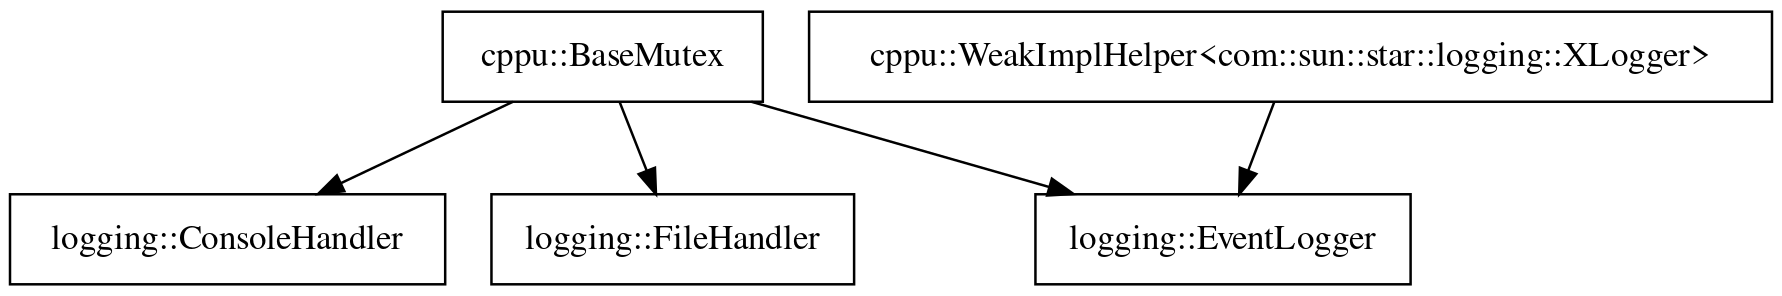
\includegraphics[width=16cm]{libloglo_partial.png}
\caption{Partial class tree of libloglo.so from LibreOffice}
\label{libloglo}

\end{figure}

Finally, we also studied the closed-source \emph{zoom}~\cite{zoom} binary.
This test case is very interesting in two ways.
First, we found \emph{6039 classes} in the binary, with \emph{5601 edges}
in the class hierarchy graph.
Second, as a large (76M) and complex ELF file, it served as a perfect benchmark 
for the performance of the algorithm.
By adding a simple check earlier in the RTTI-spotting pipeline, we sped up the
analysis of the zoom binary 13.37 times, from over an hour to around five
minutes.

\autoref{discoverbenchmarks} details the benchmarks we conducted on many 
well-known projects.

\begin{table}[h]
  \centering
  {\small
  \begin{tabular}{l | r | r | r | r }
    ELF File and version & Size & Size of .rodata & Computation time & Amount 
of classes recovered  \\
    \hline
    gold 1.16 & 2.3M & 0.1M & 0m0.605s & 571 \\
    ceph-dencoder 15.2.13 & 29M & 0.9M & 0m12.493s & 2959 \\
    zoom 5.5.7938.0228 & 76M & 16M & 5m50.626s & 6039 
  \end{tabular}
  }

\caption{Benchmarks of dis-cover on a machine running Ubuntu 20.04 with a 2.6 
GHz dedicated vCPU}
\label{discoverbenchmarks}

\end{table}


\section{Analysis of Debian packages}
\label{debiansection}

As we have shown before, out of the 5827 Debian packages that list C++ as a 
dependency, we extracted classes from 3194 (54\%).
The total number of classes we found is 960'188, with 39\% of them unique 
across all packages (unique name in unique tree).
The mean number of classes in packages where there are classes is 300.

In \autoref{classdistribution}, we can see the graph of the number of classes
in individual packages. We excluded the 20 projects with the most classes, as
they made the graph much less readable (some packages had more then 10,000
classes).

\begin{figure}

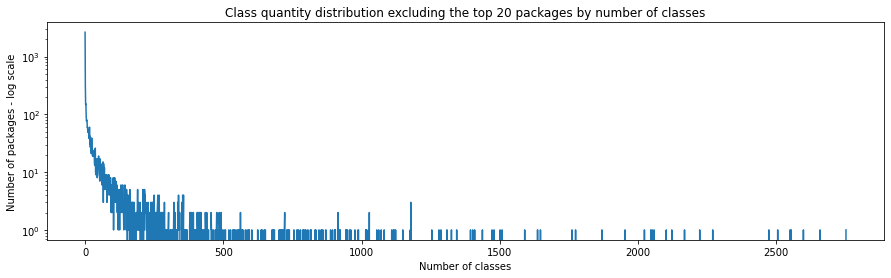
\includegraphics[width=16cm]{package_distribution.png}
\caption{Class quantity distribution in Debian packages with C++ as a
dependency (y log scale)}
\label{classdistribution}

\end{figure}

Using data from the Debian Popularity Contest~\cite{popcon} (popcon), we
analyzed the most popular packages to see if the numbers evolved.
In \autoref{toppackages} you can examine our results.
We can observe there are more classes (more frequently and in greater numbers)
in the most popular Debian packages then in the overall population of Debian
packages.

\begin{table}[h]
  \centering
  {\small
  \begin{tabular}{r | l | r | r}
    Number of packages & Sorting criteria & Percentage of packages & Mean 
    number of classes \\
    & & with classes recovered & per package with classes \\
    \hline
    100 & usage & 71\% & 330 \\
    100 & installations & 61\% & 356 \\
    1000 & usage & 64\% & 171 \\
    1000 & installations & 61\% & 169 \\
    5827 & - & 54\% & 300
  \end{tabular}
  }

\caption{Class statistics on the most popular packages of Debian}
\label{toppackages}

\end{table}


\section{Testing RetroWrite}

We were able to test the new C++ capabilities of RetroWrite on examples we had
coded ourselves.
% TODO modify this if it changes
The tool did not yet manage to rewrite larger projects.
This will be fixed before we make the code public.

Also, testing on well-known closed-source projects proved an issue, because
the binaries were stripped, and thus the function boundaries were not known.
RetroWrite does not yet support unstripped binaries because of this.
In order to make RetroWrite work on projects such as Chrome~\cite{chrome} or
Zoom~\cite{zoom}, one could use a function identification tool such as the
ones found in IDA Pro~\cite{ida} or radare2~\cite{radare}.
These tools use heuristics to find the function boundaries, so they might not
work for every project.

\lou{TODO say we tried more complex code, not just simple examples}


%%%%%%%%%%%%%%%%%%%%%%
\chapter{Related Work}
%%%%%%%%%%%%%%%%%%%%%%

% The related work section covers closely related work. Here you can highlight
% the related work, how it solved the problem, and why it solved a different
% problem. Do not play down the importance of related work, all of these
% systems have been published and evaluated! Say what is different and how
% you overcome some of the weaknesses of related work by discussing the 
% trade-offs. Stay positive!

% This section is usually 3-5 pages.


\section{MARX}
\label{relatedworksmarx}

MARX~\cite{marx} is a static analysis tool which is related to what dis-cover
is trying to achieve. Using analysis of the virtual tables in a C++ binaries,
they accurately extract 90\% of the classes. This is done without the need for
RTTIs, and thus can target a larger number of projects (such as the chrome
browser and the Node.js runtime) at the cost of having a probabilistic
approach.

In comparison, dis-cover can recover 100\% of the classes present in a binary,
but only if the RTTIs were kept at compilation time (so no class can be
recovered from the chrome browser and the Node.js runtime).

MARX uses six heuristics to locate the virtual tables, related to the table
layout and content.

This project could be a great candidate for future integration into
RetroWrite, if we extend the tool to add defenses around type integrity for
example.


\section{Plugins}

There exists multiple plugins for reverse engineering frameworks that serve
the same purpose as dis-cover. For IDA Pro, there exists \emph{IDA GCC RTTI}
~\cite{idagccrtti}, and for Ghidra there is the \emph{Class and Run-Time
Type Information Analyzer}~\cite{ghidracppclassanalyzer}.

These are very useful, and integrate very well into the reverse engineering
frameworks, but they cannot make that information available to other tools.

The IDA Pro plugin does offer the option to create a \emph{.dot} graph file
that can be used to create a visual representation of the hierarchy tree.
Our \emph{dis-cover} tool offers the same functionality (see
\autoref{visualizingsection})

\dam{Do these plugins exactly the same as dis-cover (without DWARF output)?
Or have they less or more advanced features?}
\lou{The key here is "integrate very well into the RE frameworks". They use
these tools' built-in UI to represent the data however they want, which we
cannot do.}


\section{Type Integrity}

\subsection{CFIXX}
\label{cfixx}

\emph{CFIXX}~\cite{cfixx} introduces \emph{Object Type Integrity}, which
is a dynamic (runtime) mechanism that keeps track of object types and prevents
adversaries from overwriting type information to hijack the control flow.

Indeed, some attacks rely on overwriting the pointer to an object's virtual
table with another one, to modify the methods called by the code and tamper
with the control flow integrity of the program.
Object Type Integrity is achieved by making sure that the right virtual table is
accessed at runtime for each specific object.

A future project could use the classes extracted with dis-cover and the
rewriting capabilities of RetroWrite to implement object type integrity on
closed-source binaries.

\subsection{HexType}
\label{hextype}

\emph{HexType}~\cite{hextype} aims to remove \emph{type confusion errors}
from programs, by adding explicit runtime checks during compilation.
This is done even for objects that are not polymorphic, so as to remove all
of the attack surface.

Type confusion errors occur when a type cast is done on incompatible types.
This can then lead to errors that can be abused to attack programs and gain
control of systems.

Adding runtime checks during compilation allows for great coverage and low
overhead.


\section{Exploiting the hard-working DWARF}

\emph{Exploiting the Hard-Working DWARF}~\cite{hardworkingdwarf}
demonstrates that it is possible to incorporate exploits in the
\texttt{.eh\_frame} and \texttt{.gcc\_except\_table} sections of an ELF file.

They show that the exception handling mechanism of ELF files is a
Turing-complete language, and that they can incorporate arbitrary programs
into DWARF sections that get executed whenever an exception is thrown by the
code.
These arbitrary programs can be used to take control over the system.

This is quite interesting, as malware-finding software usually does not scan
these debug sections for malicious code, and existing reverse engineering
tools do not know how to interpret these malformed DWARF sections.

This paper rekindled a global interest in DWARF as an academic research topic,
which lead to projects like this one.

This project also shows both the power of the DWARF debugging format and the
need for more research to be done around this topic.

%%%%%%%%%%%%%%%%%%%%
\chapter{Conclusion}
%%%%%%%%%%%%%%%%%%%%

% In the conclusion you repeat the main result and finalize the discussion of
% your project. Mention the core results and why as well as how your system
% advances the status quo.

In conclusion we develop \emph{dis-cover}, a static analysis tool for C++
binaries that can find polymorphic class hierarchies without using heuristics,
if the compiler was told to keep the \emph{Run-Time Type Information}.
The tool injects its findings in the analyzed binary as DWARF debug
information and ELF symbols, so it can be used in any debugging tool.
We hope this serves as an example for future binary analysis tools.

We also extend the static position-independent binary rewriter RetroWrite with
C++ support, and [TODO].
To our knowledge, RetroWrite is the first static rewriter that can add
instrumentation like AddressSanitizer to closed-source C++ binaries that make
use of exceptions.

\cleardoublepage
\phantomsection
\addcontentsline{toc}{chapter}{Bibliography}
\printbibliography

% Appendices are optional
% \appendix
% %%%%%%%%%%%%%%%%%%%%%%%%%%%%%%%%%%%%%%
% \chapter{How to make a transmogrifier}
% %%%%%%%%%%%%%%%%%%%%%%%%%%%%%%%%%%%%%%
%
% In case you ever need an (optional) appendix.
%
% You need the following items:
% \begin{itemize}
% \item A box
% \item Crayons
% \item A self-aware 5-year old
% \end{itemize}

\end{document}
